\documentclass[11pt]{article}


\usepackage{amsmath}
\usepackage{fixmath}
\usepackage{bm}
\usepackage{tikz}
\usetikzlibrary{automata,positioning,calc}
\usepackage{listings}
\renewcommand{\lstlistingname}{Code}% Listing -> Algorithm
\renewcommand{\lstlistlistingname}{List of \lstlistingname s}% List of Listings -> List of Algorithms
\usepackage{color}
\usepackage{xcolor}
\usepackage{textcomp}
\usepackage{graphicx}
\usepackage{soul}
\usepackage{amsfonts,amsmath}
\usepackage{latexsym}
\usepackage{fullpage}
\usepackage{graphicx}
\usepackage[bottom]{footmisc}
\usepackage{soul}
\usepackage{color}
\usepackage{mathtools}
\usepackage{fancybox}
\usepackage{tikz}
\usetikzlibrary{shapes.multipart}
 
\definecolor{codegreen}{rgb}{0,0.6,0}
\definecolor{codegray}{rgb}{0.5,0.5,0.5}
\definecolor{codepurple}{rgb}{0.58,0,0.82}
\definecolor{backcolour}{rgb}{0.95,0.95,0.92}
 
\lstdefinelanguage{JavaScript}{
  keywords={break, case, catch, continue, debugger, default, delete, do, else, false, finally, for, function, if, in, instanceof, new, null, return, switch, this, throw, true, try, typeof, var, void, while, with},
  morecomment=[l]{//},
  morecomment=[s]{/*}{*/},
  morestring=[b]',
  morestring=[b]",
  ndkeywords={class, export, boolean, throw, implements, import, this},
  keywordstyle=\color{blue}\bfseries,
  ndkeywordstyle=\color{darkgray}\bfseries,
  identifierstyle=\color{black},
  commentstyle=\color{purple}\ttfamily,
  stringstyle=\color{red}\ttfamily,
  sensitive=true
} 
 
\lstdefinestyle{mystyle}{
    backgroundcolor=\color{backcolour},   
    commentstyle=\color{codegreen},
    keywordstyle=\color{magenta},
    numberstyle=\tiny\color{codegray},
    stringstyle=\color{codepurple},
    basicstyle=\footnotesize,
    breakatwhitespace=false,         
    breaklines=true,                 
    captionpos=b,                    
    keepspaces=true,                 
    numbers=left,                    
    numbersep=5pt,                  
    showspaces=false,                
    showstringspaces=false,
    showtabs=false,                  
    tabsize=2
}
 
 
\lstset{style=mystyle}

\newenvironment{code}{\begin{tabbing}
    12345\=12345\=12345\=12345\=12345\=12345\=12345\=12345\= \kill }
  {\end{tabbing}}

\usepackage{stmaryrd}
\usepackage[T1]{fontenc}  % access \textquotedbl

\newcommand{\hlc}[2][yellow]{{%
    \colorlet{foo}{#1}%
    \sethlcolor{foo}\hl{#2}}%
}

\title{%
  Recitation Note 2 \\
  \large CSCI-GA.2110-001 Programming Languages}
\date{\today}
\author{Yusen Su}


\begin{document}
\maketitle
\section{Scoping}
\subsection{Definition}
\begin{itemize}
\item Binding: a binding is an association of two things. Example: binding a variable name with a value.
\item Static Binding: name binding performed before the program is running (compile time).
\item Dynamic Binding: name binding performed when the program is executing (running time).
\item Scope: the region of program text where a binding is active.
\item Static Scoping: binding of a name is determined by rules that refer only to the program text (i.e. its syntactic structure).
\item Dynamic Scoping: binding of a name is given by the most recent declaration encountered during run-time.
\item Nested scopes:  given nested subroutines (e.g. blocks, classes), the scope for a nested subroutine is inside another scope.  \\
Typically, bindings created inside a nested scope are not available outside that scope.

\end{itemize}
\subsection{How to consider the variable bindings under static/dynamic scoping in the code segment?}
Global variable: declare outside any functions, could be accessed on any functions.\\
Local variable: declare inside a function, could only be accessed by that function.\\
Variable shadowing (hide): In a certain scope, if you redeclare a variable, the original binding is hidden, and has a hole in its scope.\\
\begin{itemize}
\item Static Scoping: depends on the code structure. The variable is bound by a data structure like tree. The nearest variable declaration of that variable in the code hierarchy (same level or upper levels).
\item Dynamic Scoping: depends on the execution order. The variable is bound by a data structure like stack. The nearest variable declaration of that variable in the running order hierarchy (same level or upper levels).
\end{itemize}
For example, consider this code segment (assume variable should be declared before used):
\begin{lstlisting}[mathescape, language=JavaScript]
0: var x = 1;
1: {
		x = x + 1;
		var x = 2;
   3:{
 			x = x + 2;
 			var x = 1;
 			x = x + 1;
		 }
  }
2:{
		var y = 0;
		y = x + 1;
  }
\end{lstlisting}
For static scoping, we could generate a scoping tree based on code structure:
\begin{center}
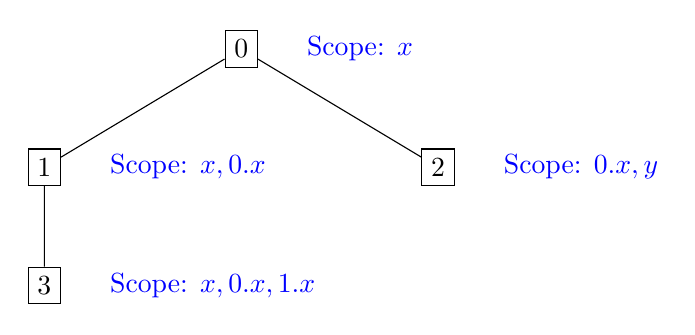
\begin{tikzpicture}[
level 1/.style={sibling distance=50mm}
]
\node [rectangle,draw] (m){$0$}
  child {node [rectangle,draw] (z) {$1$} 
  	 child {node [rectangle,draw] (z1) {$3$} }
  }
  child {node [rectangle,draw] (a) {$2$}
};
\node [blue, right= 5mm of m] {Scope: $x$};
\node [blue, right= 5mm of z] {Scope: $x,0.x$};
\node [blue, right= 5mm of z1] {Scope: $x,0.x,1.x$};
\node [blue, right= 5mm of a] {Scope: $0.x, y$};
\end{tikzpicture}
\end{center}
For dynamic scoping, we could generate a scoping stack based on running order:
\begin{itemize}
\item consider the program is executing at line 8:
\begin{figure}[hbt!]
  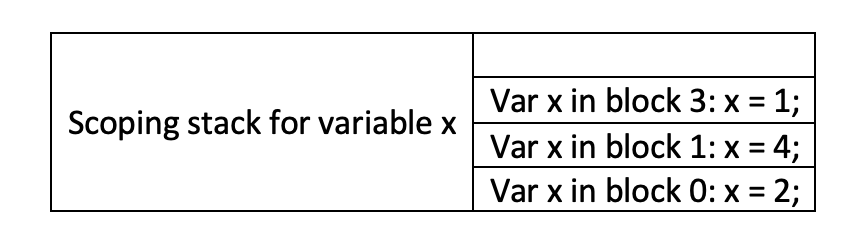
\includegraphics[scale = 0.5]{lin8.png}
  \label{fig:correct}
\end{figure}
\item scope stack example when the program is running at line 10:
\begin{figure}[hbt!]
  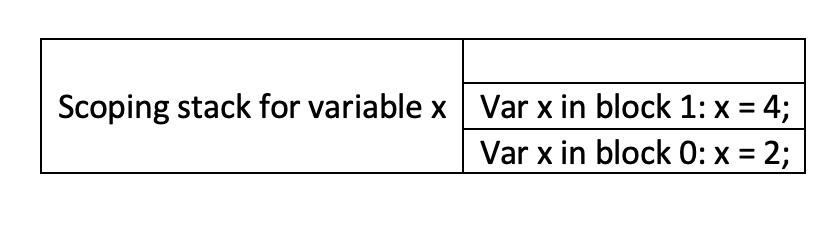
\includegraphics[scale = 0.5]{lin10.png}
  \label{fig:correct}
\end{figure}
\end{itemize}

\subsection{Sample question}
Consider the following program (variable should be declared before used):
\begin{lstlisting}[mathescape, language=c++]
int x = 2;

void f(){
    int x = 3;
}

int g(){
    f();
    return x + 4;
}

int h(){
    int x = 5;
    return g();
}

printf("function g returns %d", g());
printf("function h returns %d", h());
\end{lstlisting}
\subsubsection{Assume program will run under static scoping, what does this program print?}
\textbf{Solution:} \\
function g returns 6\\
function h returns 6
\subsubsection{Assume program will run under dynamic scoping, what does this program print?}
\textbf{Solution:} \\
function g returns 6\\
function h returns 9

\section{Control Flow}
\subsection{Code components}
\subsubsection{Expression}
1. Definition: a combination of one or more constants, variables, operators, and functions that the programming language interprets and computes.\\
2. Evaluation order:
\begin{itemize}
\item Operator precedence: The order in which different infix operators are evaluated in an expression.
\item Operator association: The order in which two consecutive infix operators with same precedence in an expression.\\
	Left-associative --- evaluate from left to right
\end{itemize}
\subsubsection{Statement}
1. Definition: instructs the computer to take a specific action (usually a combination of the sequences of expressions).\\
2. Examples:\\
\begin{center}
\begin{tabular}{ |l|l|} 
 \hline
 Forms & Example \\ 
  \hline
 Assignment & $x:=5;$ \\ 
  \hline
 If statements & If ($expression$) then $statements_1$ else $statements_2$\\ 
 \hline
\end{tabular}
\end{center}
\subsection{Sequencing}
Definition: execution statement and evaluation expression in sequential (or explicit specified) order.
\subsection{Selection}
1. Definition: executing one of two statements according to the value of a Boolean expression.\\
2. Short circuit evaluation: given a Boolean expression ($x == 0$ || $y > 0$), the second argument will not be evaluated if the first condition meets.
\subsection{Iteration}
1. Definition: execute a piece of statements repeatedly.\\
2. Breaking out: early exits the loop.
\subsection{Questions}
1. Why not using unstructured control flow mechanism such as $goto$ in the modern programming language?\\
\textbf{ Sample answer:}\\
Using $goto$ is harmful because it could arrive at any particular locations of the code. It will break down the programming logic.
\end{document}